\documentclass{beamer}
\usepackage[utf8]{inputenc}
\usepackage{graphicx}
\author[Sowmya Vajjala]{Instructor: Sowmya Vajjala}

\title[LING 410X]{LING 410X: Language as Data}
\subtitle{Semester: Spring '18}

\date{27 March 2018}

\institute{Iowa State University, USA}
%%%%%%%%%%%%%%%%%%%%%%%%%%%

\begin{document}

\begin{frame}\titlepage
\end{frame}

\begin{frame}
\frametitle{Class Outline - Topic Modeling in detail}
\begin{itemize}
\item Continuing from last class: how does a topic model "learn"?
\item Sensitivity of topic model to its parameters (e.g., num. iterations)
\item Evaluating topic models automatically
\item Human evaluation of topic models \pause
\item Reminder: A5 submission due on 3/31. If topicmodels is slow, or you don't want to learn an extra library, you can also do the assignment with mallet instead. 
\end{itemize}
\end{frame}


\begin{frame}
\frametitle{Exercise on Thursday}
\begin{itemize}
\item How many of tried this out?
\item How many of you successfully make this work on your computers?
\item \pause The task was to "learn" a topic model, based on a dataset. 
\end{itemize}
\end{frame}

\begin{frame}
\frametitle{"Learning" a topic model: intuitive explanation of LDA}
\begin{itemize}
\item Aim: organize a topic collection into topics, where each topic is a collection of words.
\item Assumptions: each document is a mixture of topics, each topic is a mixture of keywords, a keyword can exist in multiple topics.
\pause \item Learning:
\begin{itemize}
\item Decide on the number of topics K. 
\item Go through each document, randomly assign each word in a document to one of the K topics. 
\item At that point, you have on poorly represented topic model already, where each document is represented as a collection of topics.
\end{itemize}
\end{itemize}
\end{frame}

\begin{frame}
\frametitle{after random initialization}
\begin{itemize}
\item Again, we start revisiting all documents. 
\item For each document d, for each word w in it, we compute two probabilities:
\\ $P(t|d)$ i.e, proportion of words in the document d assigned topic t
\\ $P(w|t)$ i.e., proportion of documents with topic t, containing word w. \pause
\item We reassign w a new topic t with a probability $P(t|d)*P(w|t)$
\item Assumption made: each time we assign a word a new topic like this, we are assuming all other assignments are correct. \pause
\end{itemize}
\end{frame}

\begin{frame}
\frametitle{Finally,}
\begin{itemize}
\item If you keep doing this process several times (iterations), you will reach a state where there is not much change in the topic-word distributions between iterations.
\item At that point, one final time, you go through all documents and assign topic probabilities to them. 
\end{itemize}
Note: Read \url{https://goo.gl/jbgCKq} for more detailed explanation of this. 
\end{frame}

\begin{frame}
\frametitle{Some name dropping}
\begin{itemize}
\item The topics and words are assumed to have "Dirichlet distribution" which is one of the several probability distributions studied in probability and statistics (D of LDA comes from there!)
\item The iterative process I conceptually explained is generally implemented by an algorithm called "Gibbs Sampling".
\end{itemize}
\end{frame}

\begin{frame}
\frametitle{"Learning" a topic model: steps in the code}
\begin{enumerate}
\item Pre-processing of the corpus (in author's version: splitting it into chunks, pre-processing of chunks)
\item Getting it into a two column format (id, text).
\item Using mallet package in R to build a topic model.
\item use mallet.import() function to convert a dataset into mallet format
\item use MalletLDA() function to create a topic model, setting its parameters. 
\item observe and analyze the output in different ways. 
\end{enumerate}
(Let me go through this taking our movie review data from text classification weeks)
\end{frame}

\begin{frame}[fragile]
\frametitle{Step 1: Pre-processing of the corpus}
\scriptsize
\begin{verbatim}
setwd("~/Dropbox/ClassroomSlides-BothCourses/LING410X/21Mar2018/data/reviews")

get_text_string <- function(file_path)
{
  fulltext <- scan(file_path, what = "character", sep = "\n")
  fulltext_as_string <- tolower(paste(fulltext, collapse = " "))
  return (fulltext_as_string)
}

files.v <- dir(path=getwd(), pattern=".*txt")
documents = c()
for(i in 1:length(files.v)){
  documents = c(documents, get_text_string(files.v[i]))
}
\end{verbatim}
\end{frame}

\begin{frame}[fragile]
\frametitle{Step 2: Getting it into a two column format (id, text)}
\scriptsize
\begin{verbatim}
docids = seq(1:length(documents))

fortopicmodels <- cbind(docids,documents)
finaldocuments <- as.data.frame(fortopicmodels, stringsAsFactors=F)
\end{verbatim}
\end{frame}

\begin{frame}[fragile]
\frametitle{Step 3: Import data into mallet}
\scriptsize
\begin{verbatim}
stoplistfile = "/ClassroomSlides-BothCourses/LING410X/21Mar2018/stoplist.csv"
mallet.instances <- mallet.import(finaldocuments$docids,
                                finaldocuments$documents,
                                stoplistfile,FALSE,token.regexp="[\\p{L}']+")
\end{verbatim}
\normalsize
\begin{itemize}
\item What does that regular expression mean? \pause It means: match one or more occurrences of any Unicode character or a " ' ". 
\item What is that "FALSE"? \pause - It is the argument "preserve case".
\end{itemize}

More on regular expressions: \url{http://www.regular-expressions.info} \\
More on unicode in regular expressions: \url{http://www.regular-expressions.info/unicode.html}
\end{frame}

\begin{frame}[fragile]
\frametitle{Setting up the topic model training process}
\footnotesize
\begin{verbatim}
topic.model <- MalletLDA(num.topics=XX) #You have to specify this.
topic.model$loadDocuments(mallet.instances) #from previous slide. 
topic.model$setAlphaOptimization(40, 80) #Optional
topic.model$train(NUM) #Actual training happens here.
\end{verbatim}
\end{frame}

\begin{frame}
\frametitle{What are all those parameters?}
\begin{itemize}
\item Best place to look for that= ?MalletLDA 
\item setAlphaOptimization(40,80) means: perform model optimization after every 40 iterations, starting first after 80 iterations. 
\item number of iterations: the more the better, generally. However, trade off is that training becomes very slow. 
\item Every 50 iterations, R prints a summary of your topic model showing top 7 words per topic. 
\item Every 10 iterations, R also shows a log likelihood of this topic model (the closer to 0, the better).
\end{itemize}
\end{frame}

\begin{frame}
\frametitle{}
\centering
\Large{Output screenshots for Thursday's Data, when I trained it last year}
\end{frame}

\begin{frame}
\frametitle{Output screenshot - at the beginning}
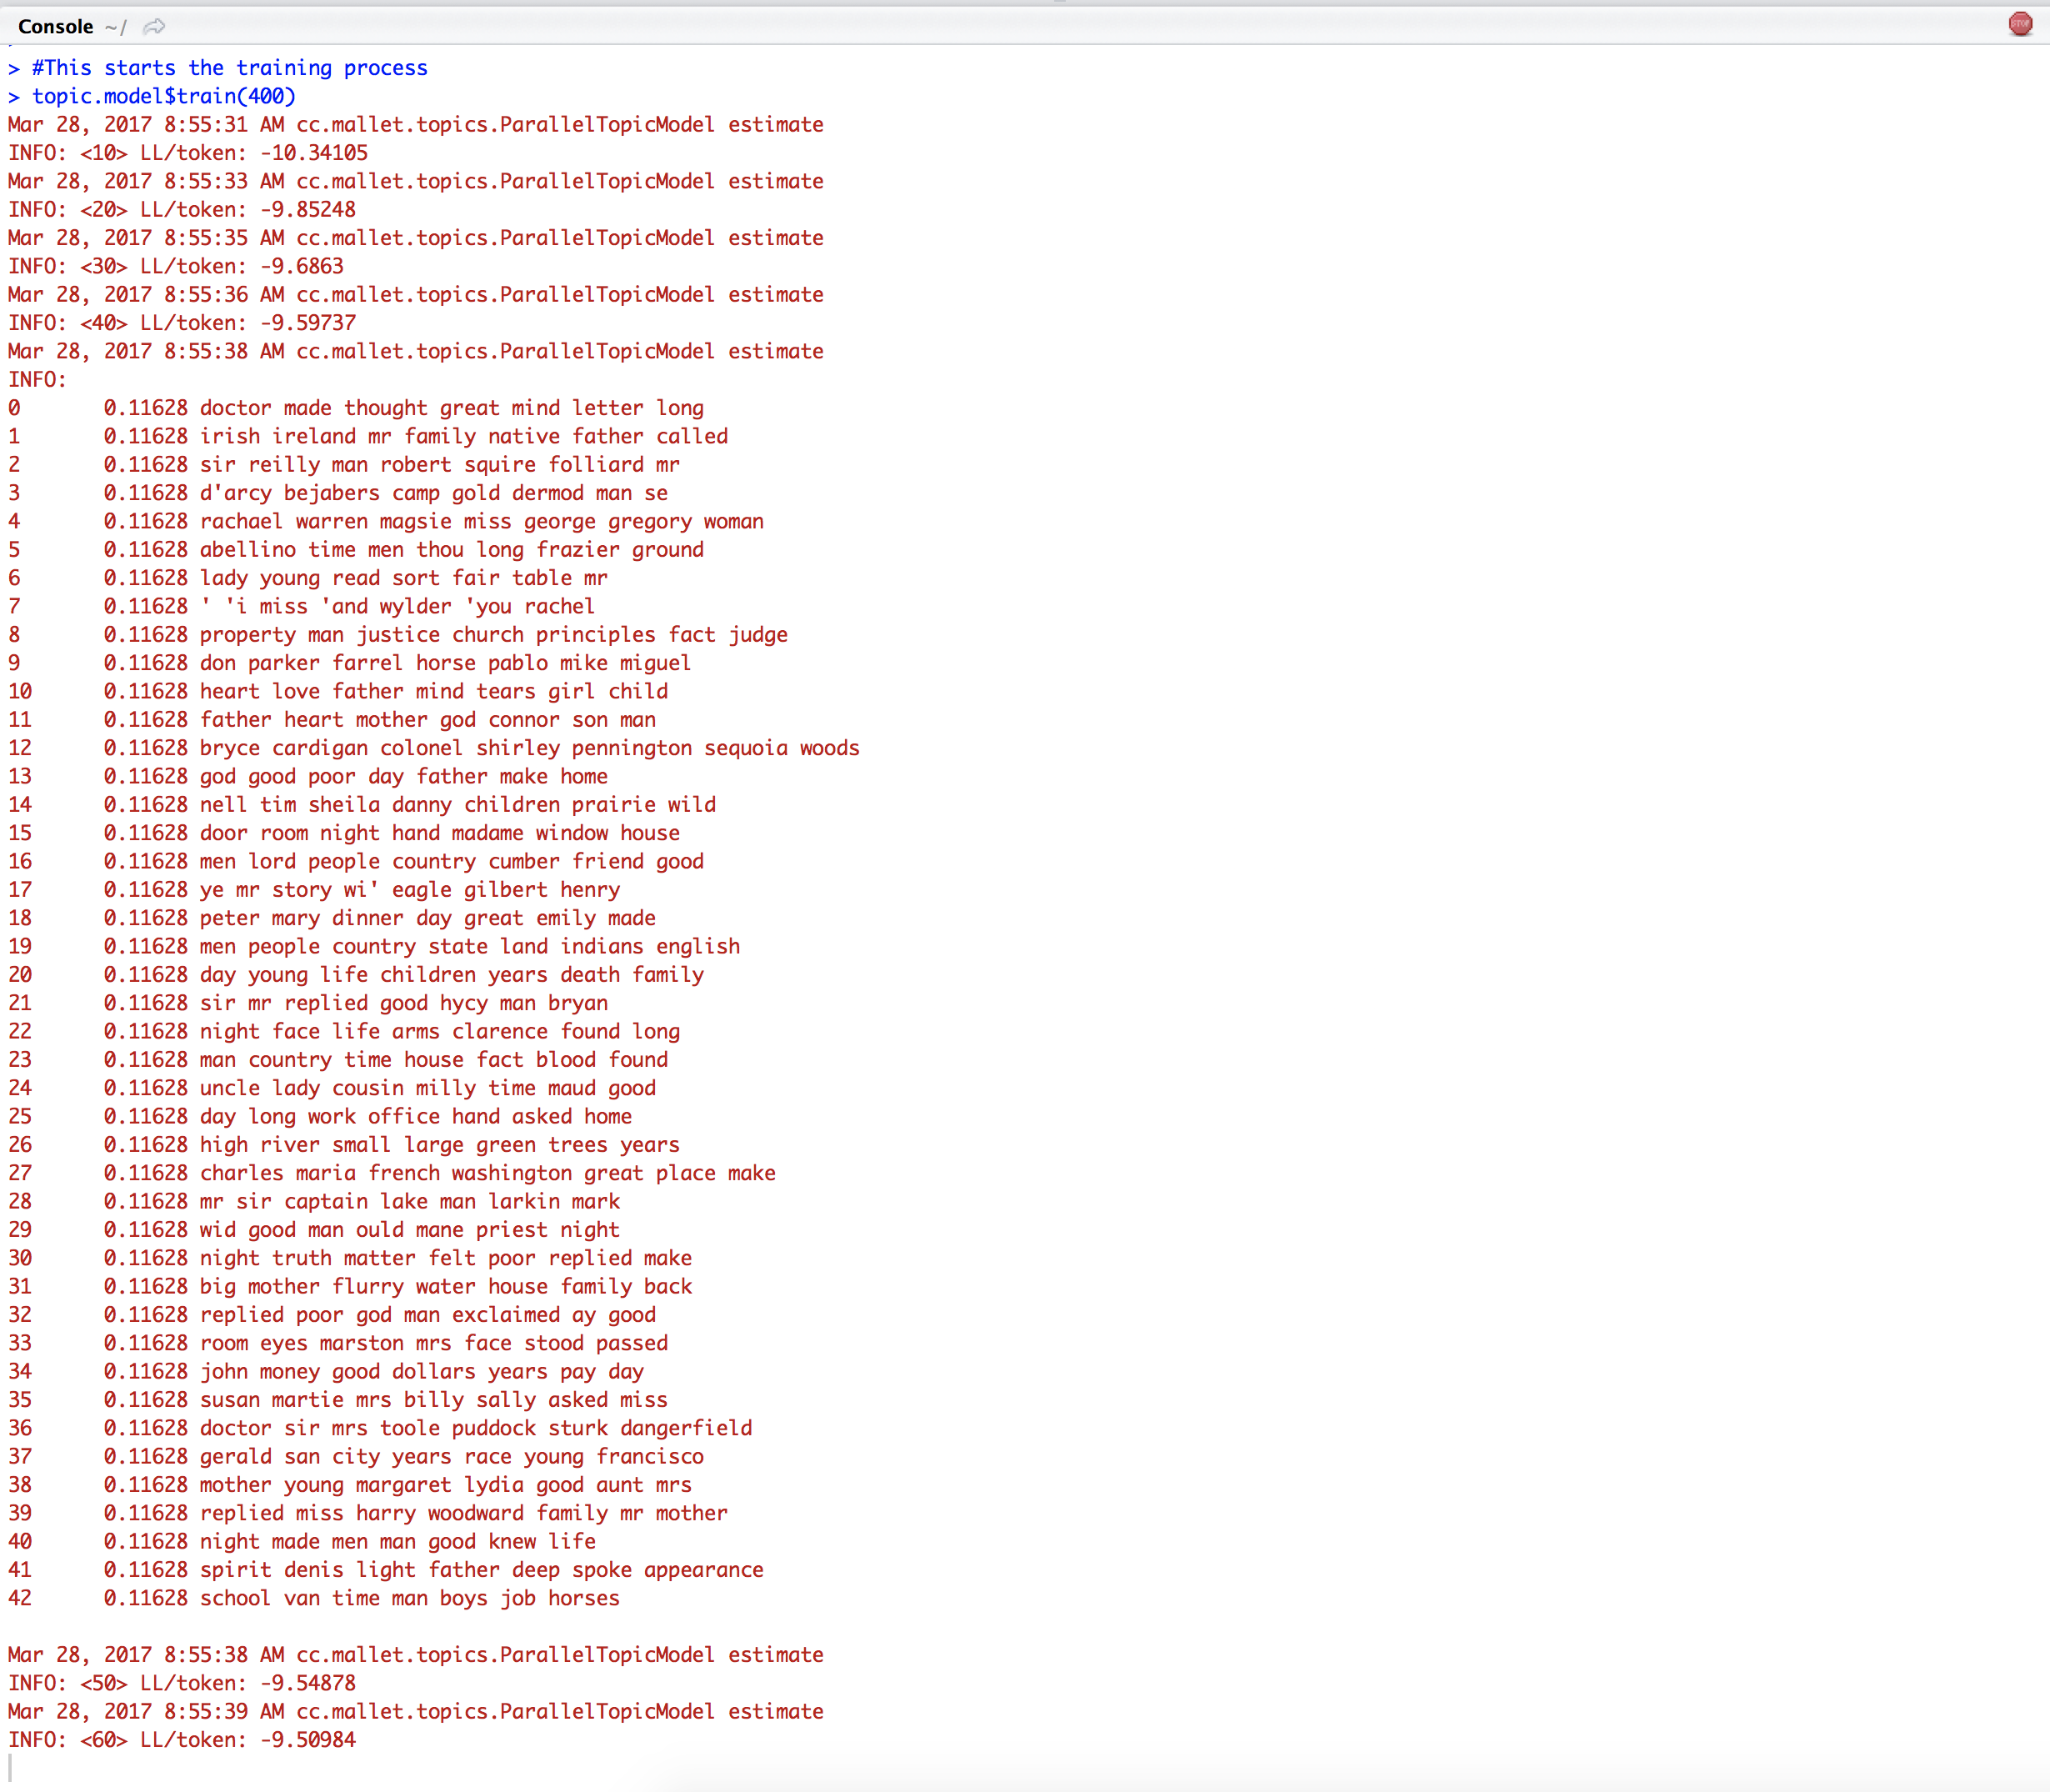
\includegraphics[width=0.8\textwidth]{topicsoutput.png}
\end{frame}

\begin{frame}
\frametitle{Output screenshot - after 400 iterations}
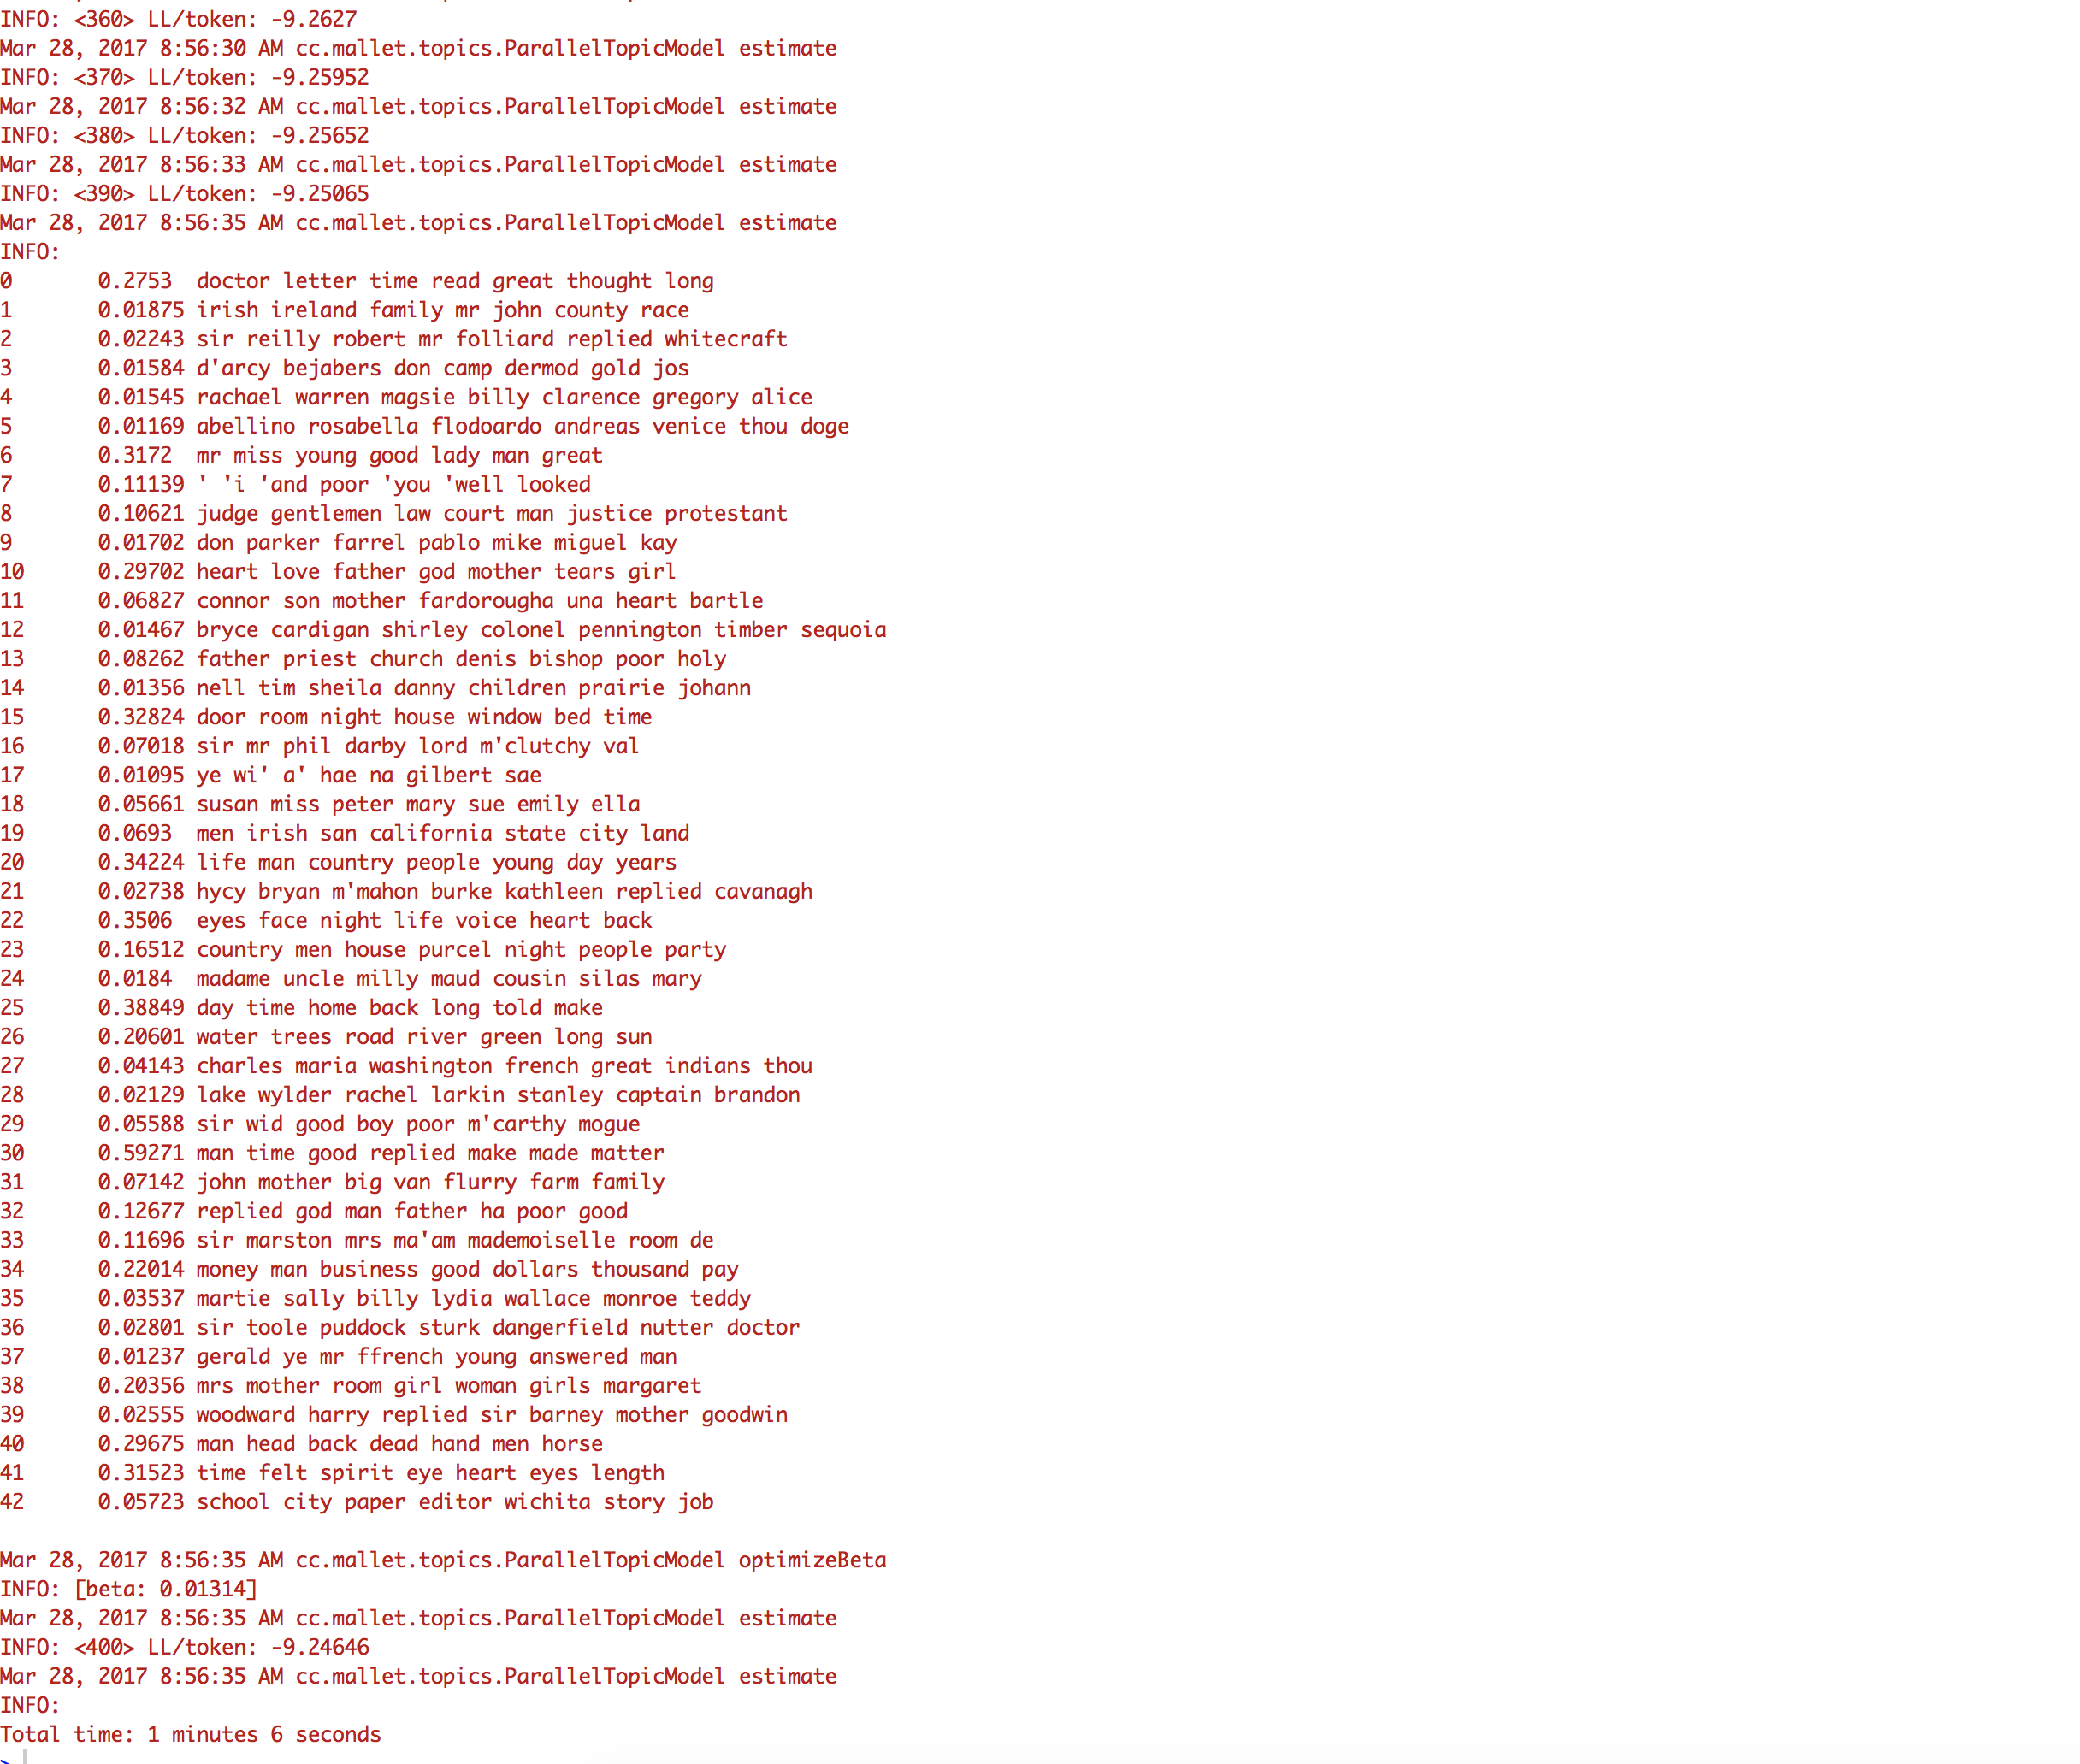
\includegraphics[width=0.8\textwidth]{topicsoutput-final.png}
\end{frame}

\begin{frame}
\frametitle{Output screenshot - 10 topics instead of 43}
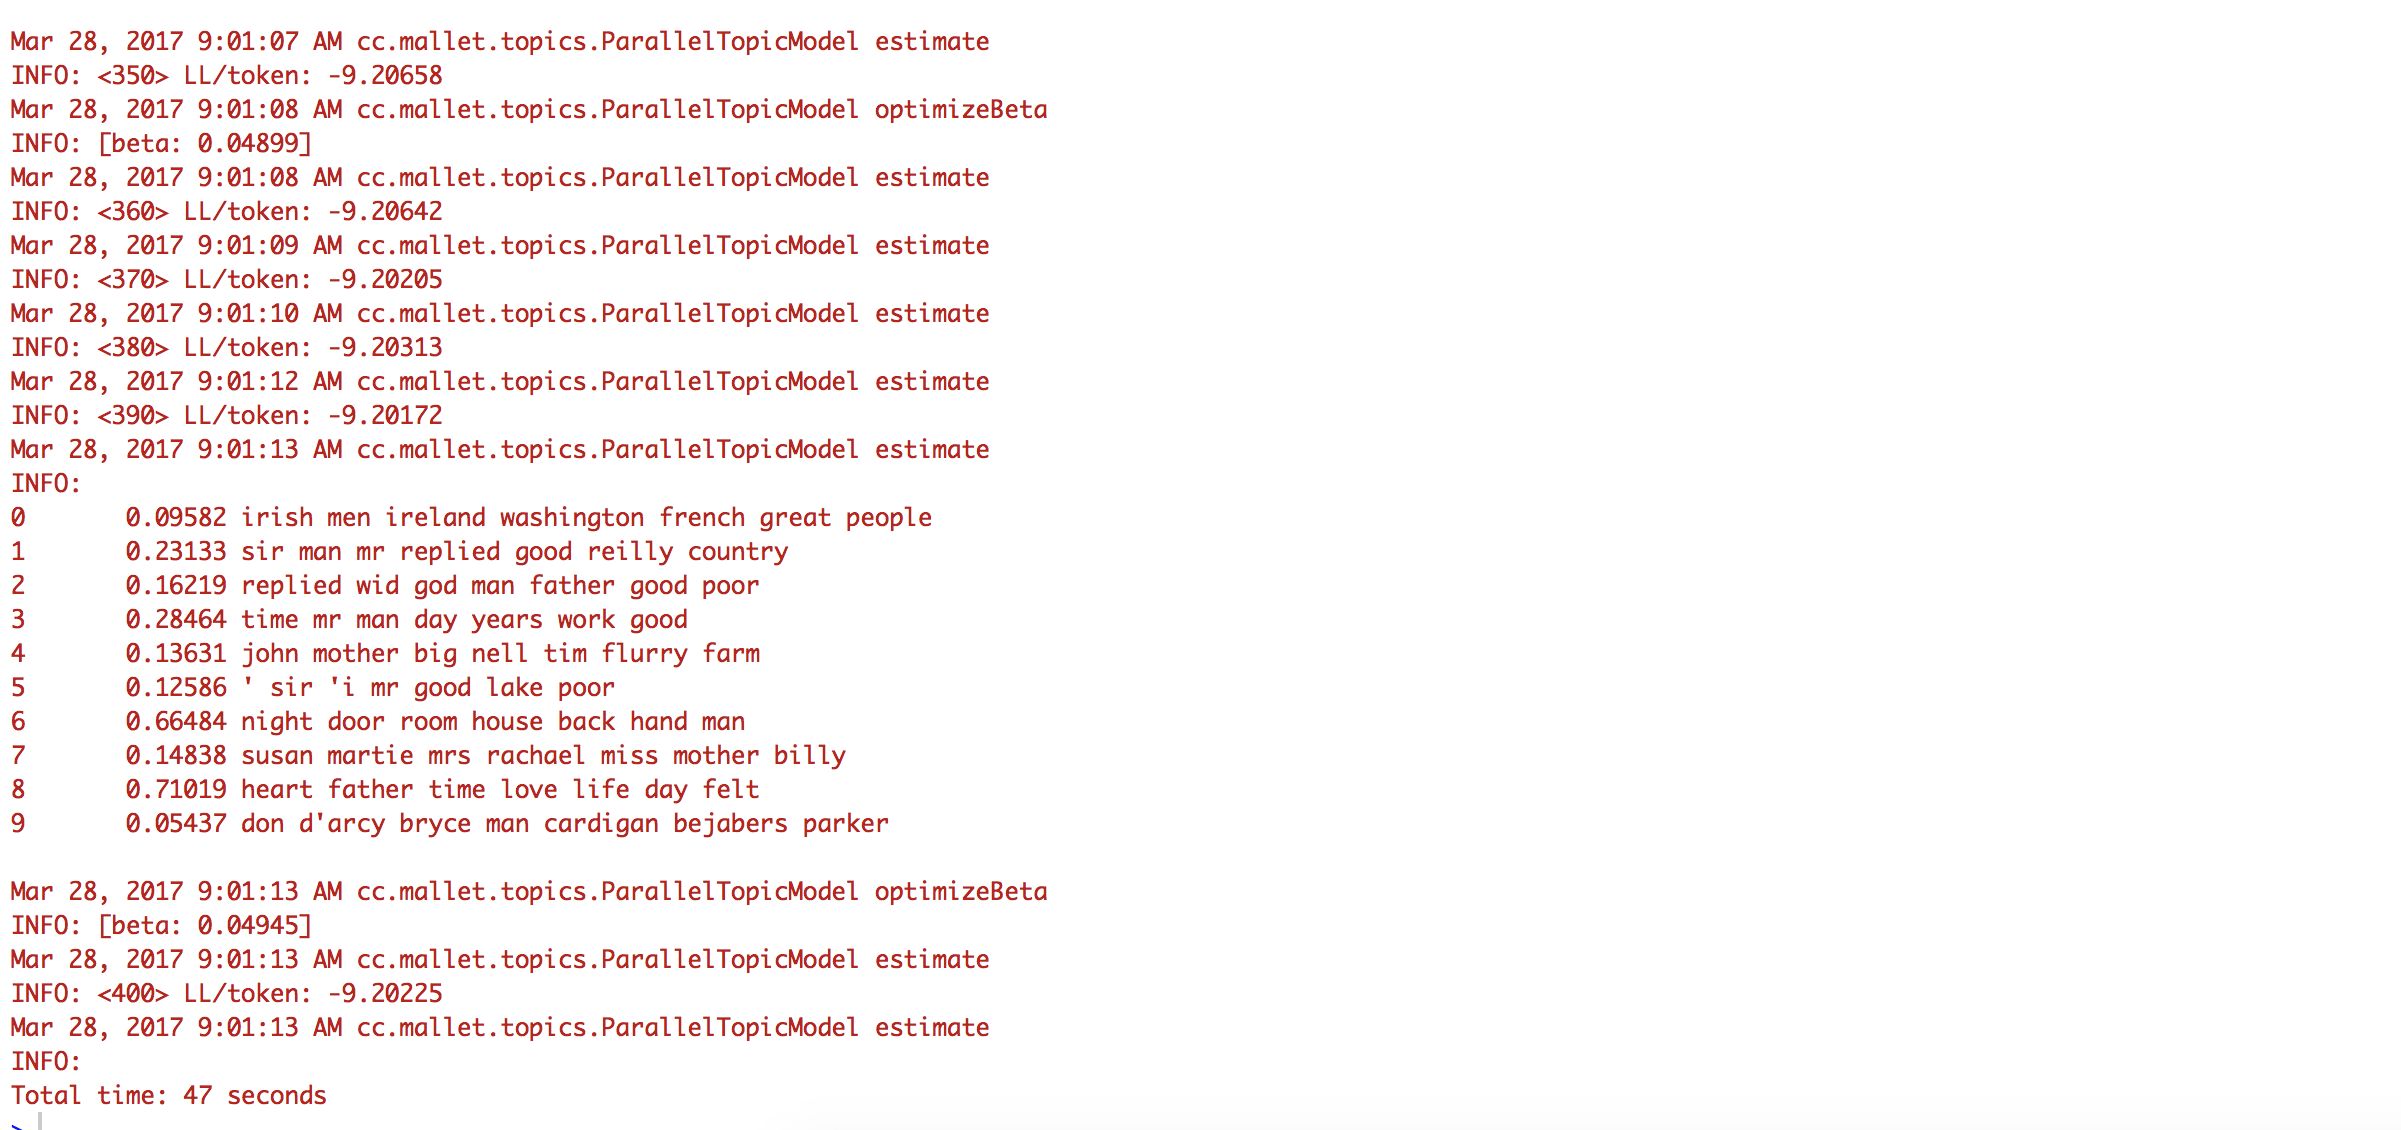
\includegraphics[width=0.8\textwidth]{topicsoutput-10topics.png}
\end{frame}

\begin{frame}
\frametitle{More functionalities in Mallet}
\begin{itemize}
\item mallet.doc.topics function returns topic weights for each document in the training data. 
\item mallet.read.dir function takes a folder path with .txt files and converts it into id-text format for mallet.
\item mallet.topic.hclust function performs a clustering of topics. 
\item mallet.topic.labels function gives a string with most probable words for a topic.
\end{itemize}
\footnotesize More details: \url{https://cran.r-project.org/web/packages/mallet/mallet.pdf}
\end{frame}

\begin{frame}[fragile]
\frametitle{Getting Topics and Words}
\footnotesize
\begin{verbatim}
doc.topics <- mallet.doc.topics(topic.model, smoothed=T, normalized=T)
\end{verbatim}
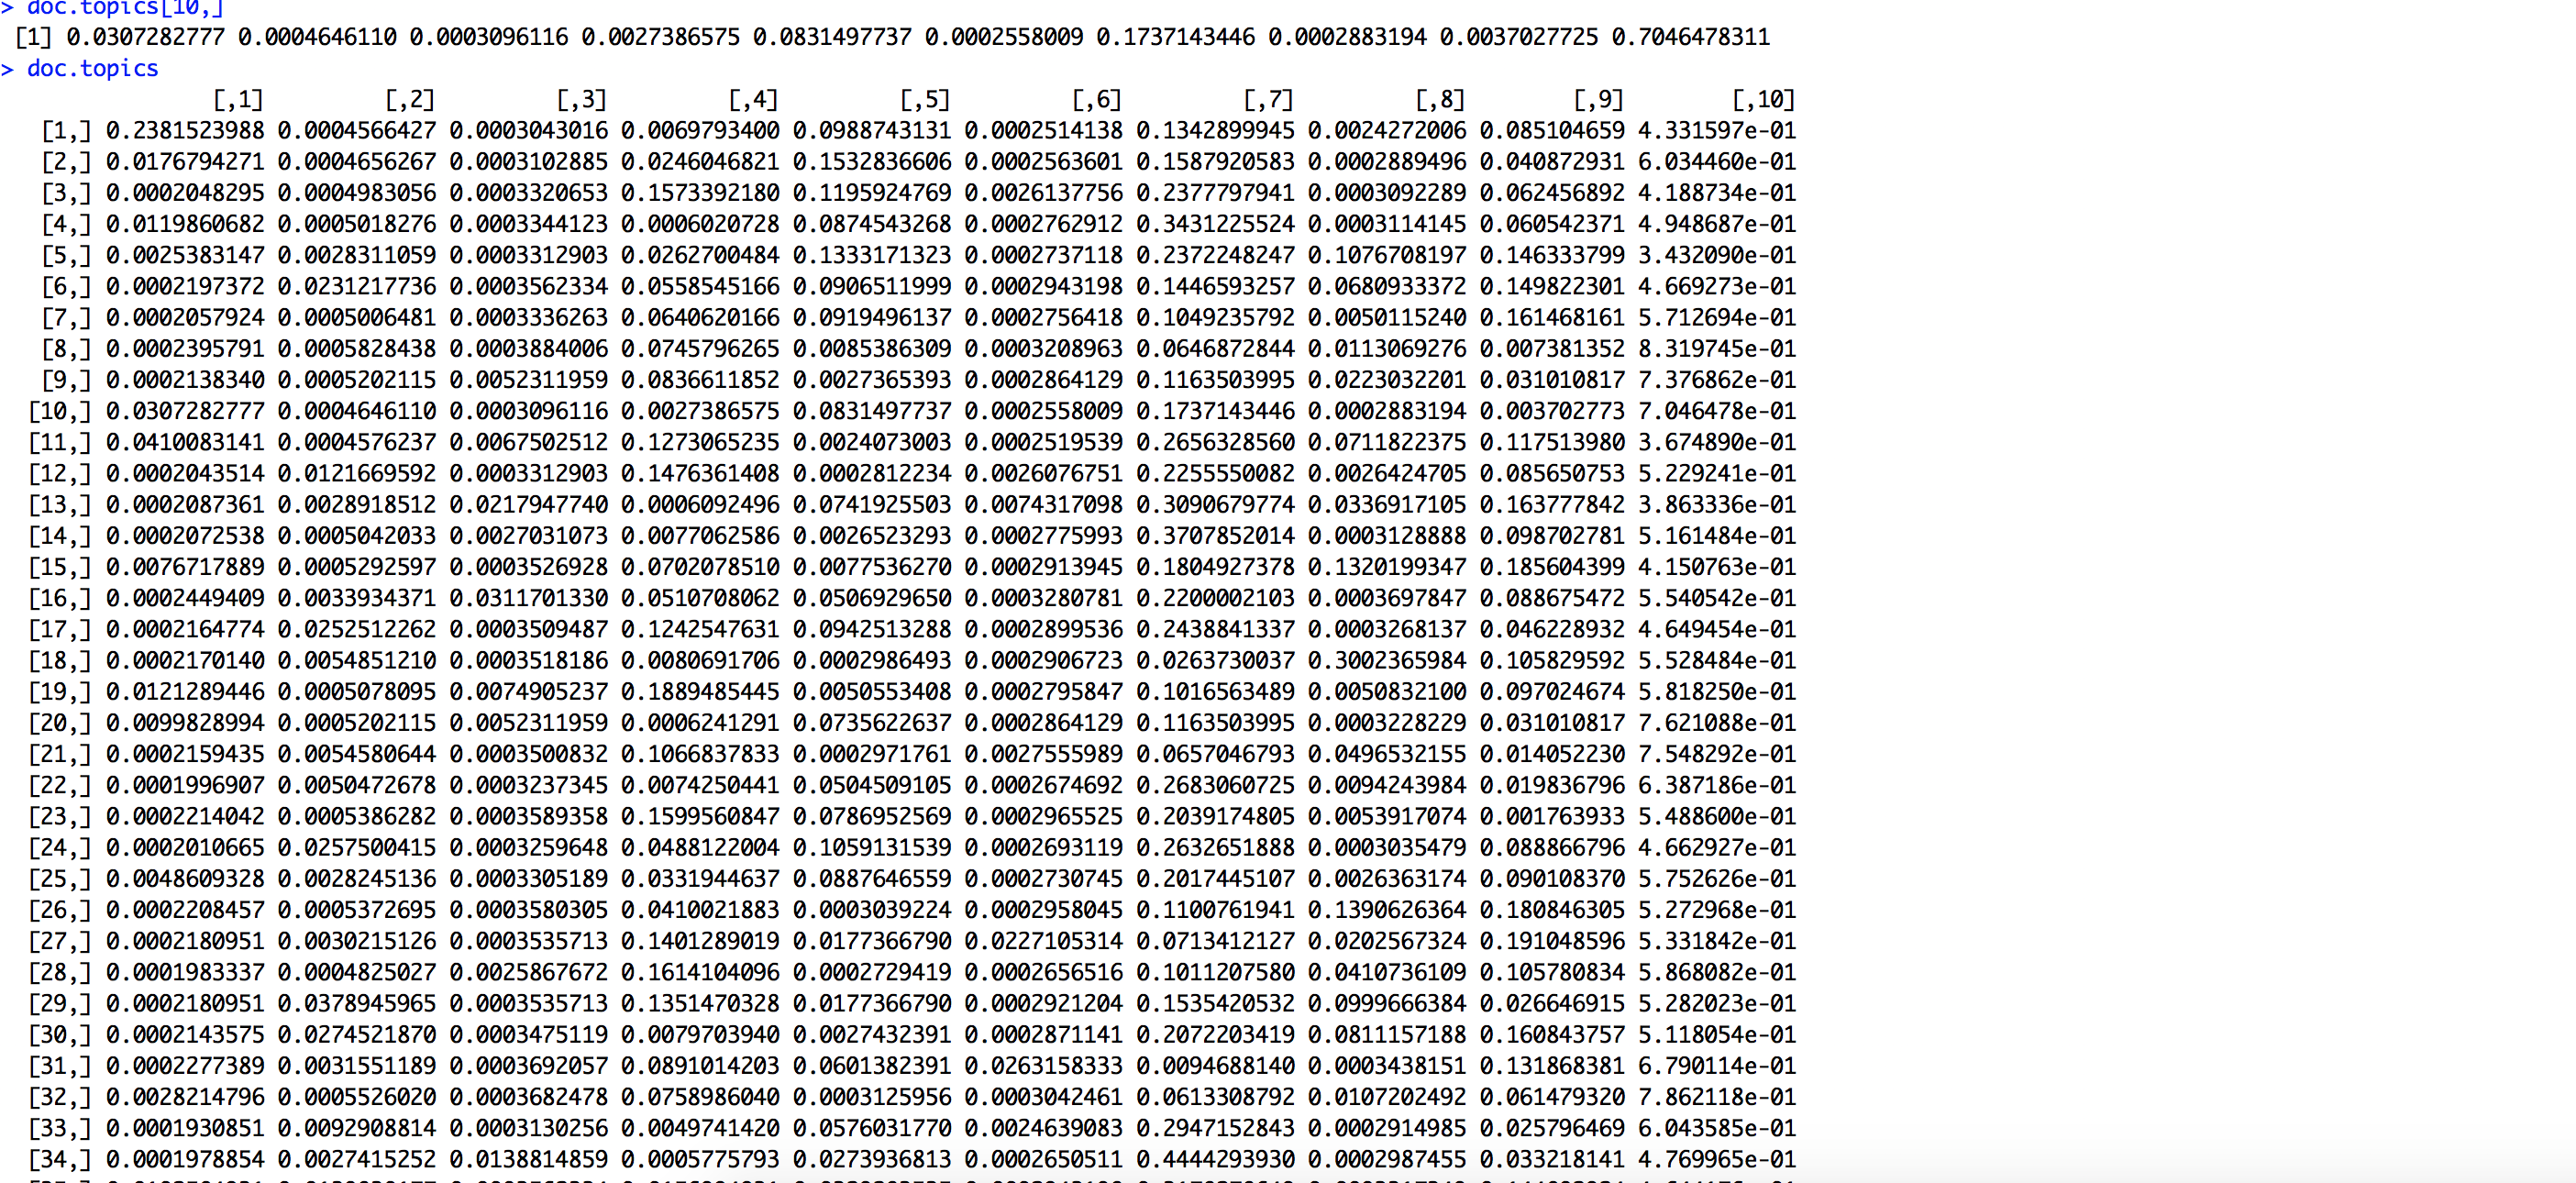
\includegraphics[width=0.8\textwidth]{doctopics.png}
\end{frame}

\begin{frame}
\frametitle{Sensitivity of a topic model to its parameters}
\begin{itemize}
\item Note: Topic models are very sensitive to their parameters.
\item How to choose the number of topics?: Intuitive - needs an understanding of the corpus. There are some ways of using probability based estimates (which are beyond the scope of this course), but there is no "formula" for choosing the best number. \pause
\item How to choose the number of iterations?: Looking at log likelihoods is a good way. 
\end{itemize}
\footnotesize Useful reference: ldatuning library in R \\ \url{https://cran.r-project.org/web/packages/ldatuning/ldatuning.pdf}
\end{frame}

\begin{frame}
\frametitle{Human evaluation of topic models -1}
\begin{itemize}
\item Word intrusion test: If an irrelevant word is shown along with related words for a given topic, a human evaluator should be able to identify that word as an intruder. \pause
\item If a human is having a difficulty doing that, the topic is not coherent. \pause
\item Experimental results: models with a larger number of topics may improve automated evaluations but will reduce human interpretability, because they will not be coherent.
\end{itemize}
\end{frame}

\begin{frame}
\frametitle{Human evaluation of topic models -2}
\begin{itemize}
\item Topic intrusion test: If a document is given, and its most appropriate topics (according a topic model) are shown along with a random topic, human evaluator should be able to identify the intruder topic correctly. \pause
\item If topic assignments from the model are intuitive, then the human intruder should not have difficulties in doing this. \pause
\item topic here means top-N keywords from the topic model for that topic. \pause
\item Experimental results: humans do well documents which have focussed discussions since it is easy to assign a topic in such cases (easy for machines too!) 
\end{itemize}
\end{frame}

\begin{frame}
\frametitle{Automatic evaluation of topic models-1}
\begin{enumerate}
\item Approximating the word intrusion test automatically by comparing semantic relatedness between words in a topic. \pause 
\item hold out a few words from each document from training data and use it to evaluate the topic model. 
\end{enumerate}
Note: Inference from a topic model is available in original Mallet tool, but does not seem to be available in the R library version. \\ \url{http://mallet.cs.umass.edu/topics.php}
\\ Enthusiasts can have a look at this R code for the same: \\ \url{https://gist.github.com/agoldst/edcfd45b5ac371296b76}
\end{frame}

\begin{frame}
\frametitle{Automatic evaluation of topic models -2}
\begin{itemize}
\item Use the topic model as a part of some other application scenario (e.g., using it to retrieve similar documents to a given document).
\item Check if the application performance has gotten better because of the use of this topic model.
\item If it does, we say the topic model is good for that application. Else, not good. \pause
\item Semi-automatic: comparing topics in terms of overlapping words in Top-25 words for each topic.
\end{itemize}
\end{frame}

\begin{frame}
\frametitle{Evaluation: general remarks}
\begin{itemize}
\item A general conclusion from topic modeling research has been that human evaluations and machine evaluations do not agree with each other. \item While machine evaluations are good for certain tasks (e.g., search engines etc.) we may need topic models that are optimized to human interpretations for some other tasks (e.g., analyzing literary documents for themes). \pause
\item One thing to keep in mind: human evaluation is expensive.
\item How to consider human interpretation as a part of the mathematical modeling process? - is an ongoing research question.
\end{itemize}
\end{frame}

\begin{frame}
\frametitle{Next Class}
\begin{itemize}
\item Wrapping up topic modeling
\item Topic modeling with or without mallet - Assignment 6 practice
\end{itemize}
\end{frame}

\end{document}
